\documentclass{article}
\usepackage{mystyle}

\title{Notes on HARDI data preprocessing: Effect on CSD fit}
\author{Scott Trinkle}
\date{Last edited: \today}

\begin{document}
\maketitle

\section{Introduction}
These notes describe the effect of HARDI data denoising on the resulting fiber
ODF (fODF) calculated using constrained spherical deconvolution (CSD) \cite{Tournier2007}. 

fODF fitting was performed using the \texttt{csdeconv} module in the
\texttt{DIPY} python package. The fiber response function was estimated from the
data using a recursive algorithm \cite{Tax2014}, initiated with a high FA mask
from the tensor fit. fODFs were then reconstructed up to a maximum spherical
harmonic degree $L_{\text{max}} = 8$, based on the recommendations of a 2013
Tournier paper \cite{Tournier2013}, which finds/claims that ``$\ell=8$ is the
highest harmonic degree that could potentially have a detectable influence on
the DW signal'' (Note: this conclusion is based on empirical analysis of
\textit{in vivo} human data with 3 mm$^3$ isotropic resolution and 500 DW
directions. We need to think through how this applies to our data.)

fODFs were calculated from the raw data, as well
as from the data denoised with sliding windows of $5\times 5\times 5$,
$7\times 7\times 7$, and $9\times 9\times 9$. As with the
\href{https://github.com/scott-trinkle/hardi/blob/master/dti/compare_denoise_widths/report/tensorfit_notes.pdf}{tensor
  fit comparison}, the volumes were not registered before computing the fODFs,
in order to isolate the effect of denoising.

\section{Comparison metrics}

\subsection{Fiber response function}

The fiber response function is defined to be symmetric about the $z$-axis, such
that its spherical harmonic representation has $c_{\ell m} = 0$ for $m \neq 0$,
where $c_{\ell m}$ is the coefficient for the real spherical harmonic function
$Y_{\ell}^m$. Figure~\ref{fig:response_sh} shows a comparison of the absolute value
of these coefficients (a proxy for ``power'' in each angular band) estimated
from the raw and denoised datasets.

\begin{figure}[h]
  \centering
  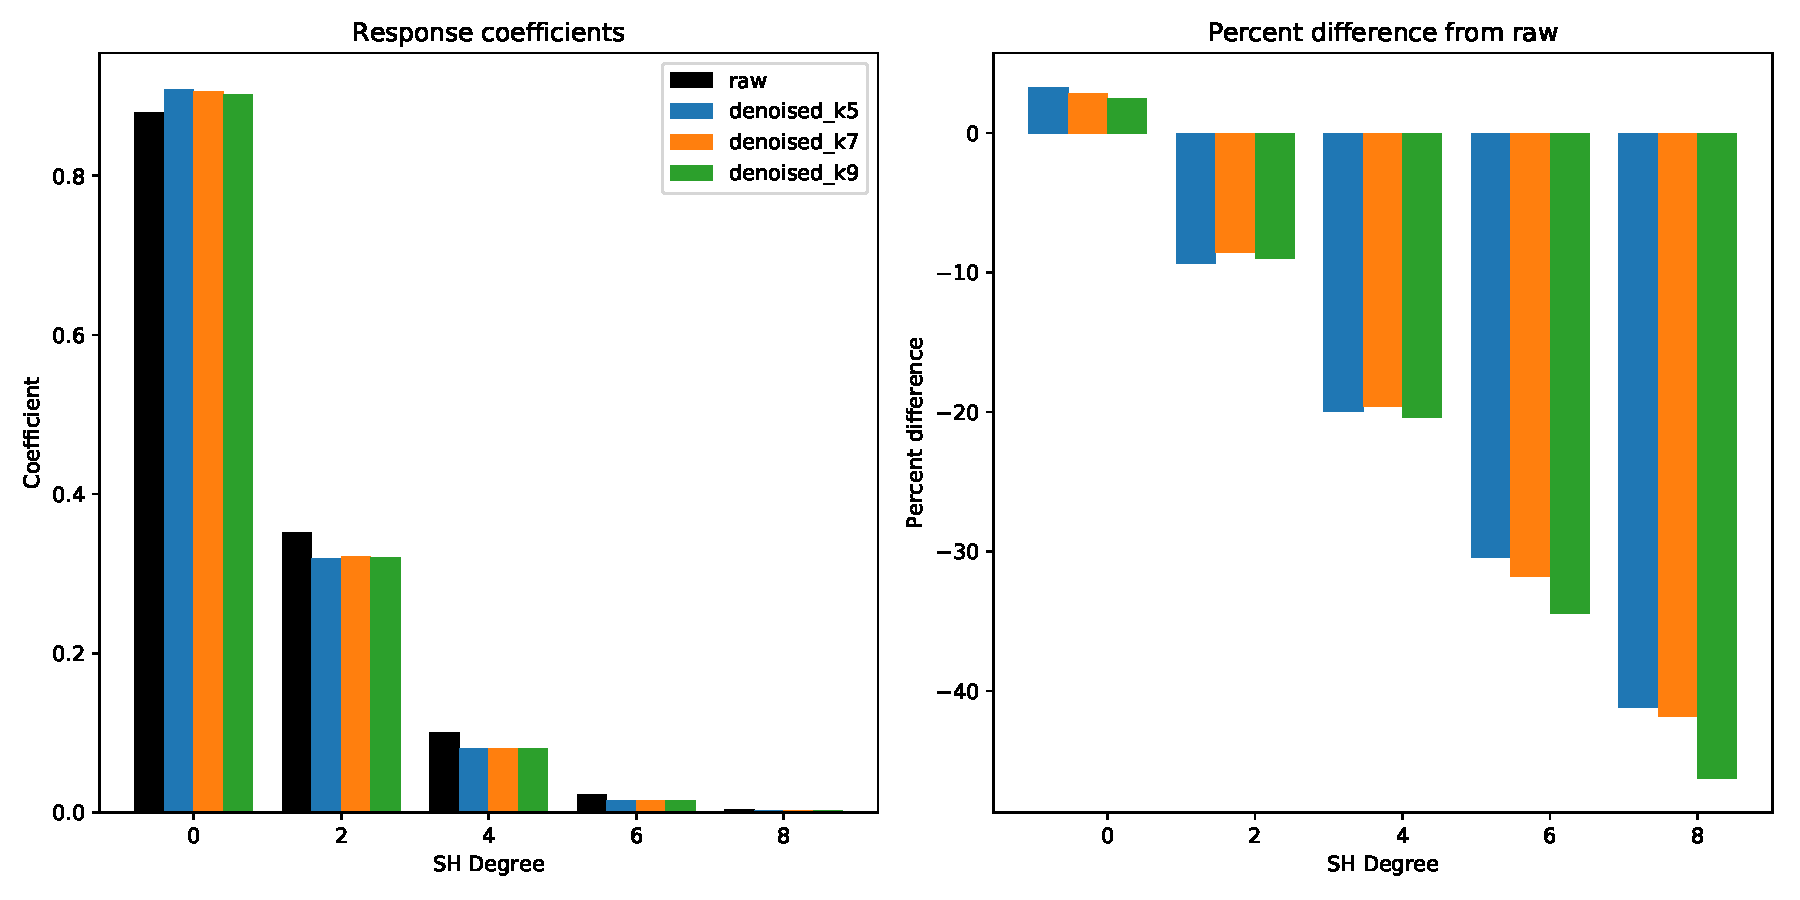
\includegraphics[width=0.8\linewidth]{../figs/response_SH}
  \captionsetup{width=0.8\linewidth}
  \caption{Left) SH representation of the fiber response functions. Right)
    percent difference between fiber response functions estimated from raw and
    denoised datasets of various window sizes.}
  \label{fig:response_sh}
\end{figure}

In general the estimated response functions are similar, though there is a
noticeable difference between the raw and denoised coefficients, which grows
more severe at higher degrees. 

\subsection{fODF scalar metrics}

Here we present comparisons of scalar metrics derived from the fODFs of the raw
and denoised data. Note that all comparisons were restricted to fODFs located
within a brain mask.

%%%%%%%%%%%%%%%%%%%%%%%%%%%%%%%%%%%%%%%%%%%%%%%%%%%%%%%%%%%%%%%%%%%%%%%%
% GFA
%%%%%%%%%%%%%%%%%%%%%%%%%%%%%%%%%%%%%%%%%%%%%%%%%%%%%%%%%%%%%%%%%%%%%%%%
\subsubsection{GFA}
Generalized fractional anisotropy (GFA) is defined as \cite{Cohen-Adad2011}:
\begin{align}
  \text{GFA} = \sqrt{\frac{N \sum_i^N{(\Psi_i - \bar{\Psi})^2}}{(N-1) \sum_i^N{\Psi_i ^ 2}}},
\end{align}
where $\Psi$ is the fODF sampled discretely at $N$ points on the unit sphere,
and the overbar denotes a mean over those sample points. Figure~\ref{fig:gfa}
shows the distribution of percent differences in GFA between the raw and
denoised fODFS, calculated as:
\begin{align}
  \text{Percent Difference} = \frac{\text{GFA}_{\text{denoised}} - \text{GFA}_{\text{raw}}}{\text{GFA}_{\text{raw}}} * 100.
\end{align}
Note that all calculations of percent difference in these notes use the same
convention presented above.

\begin{figure}[H]
  \centering
  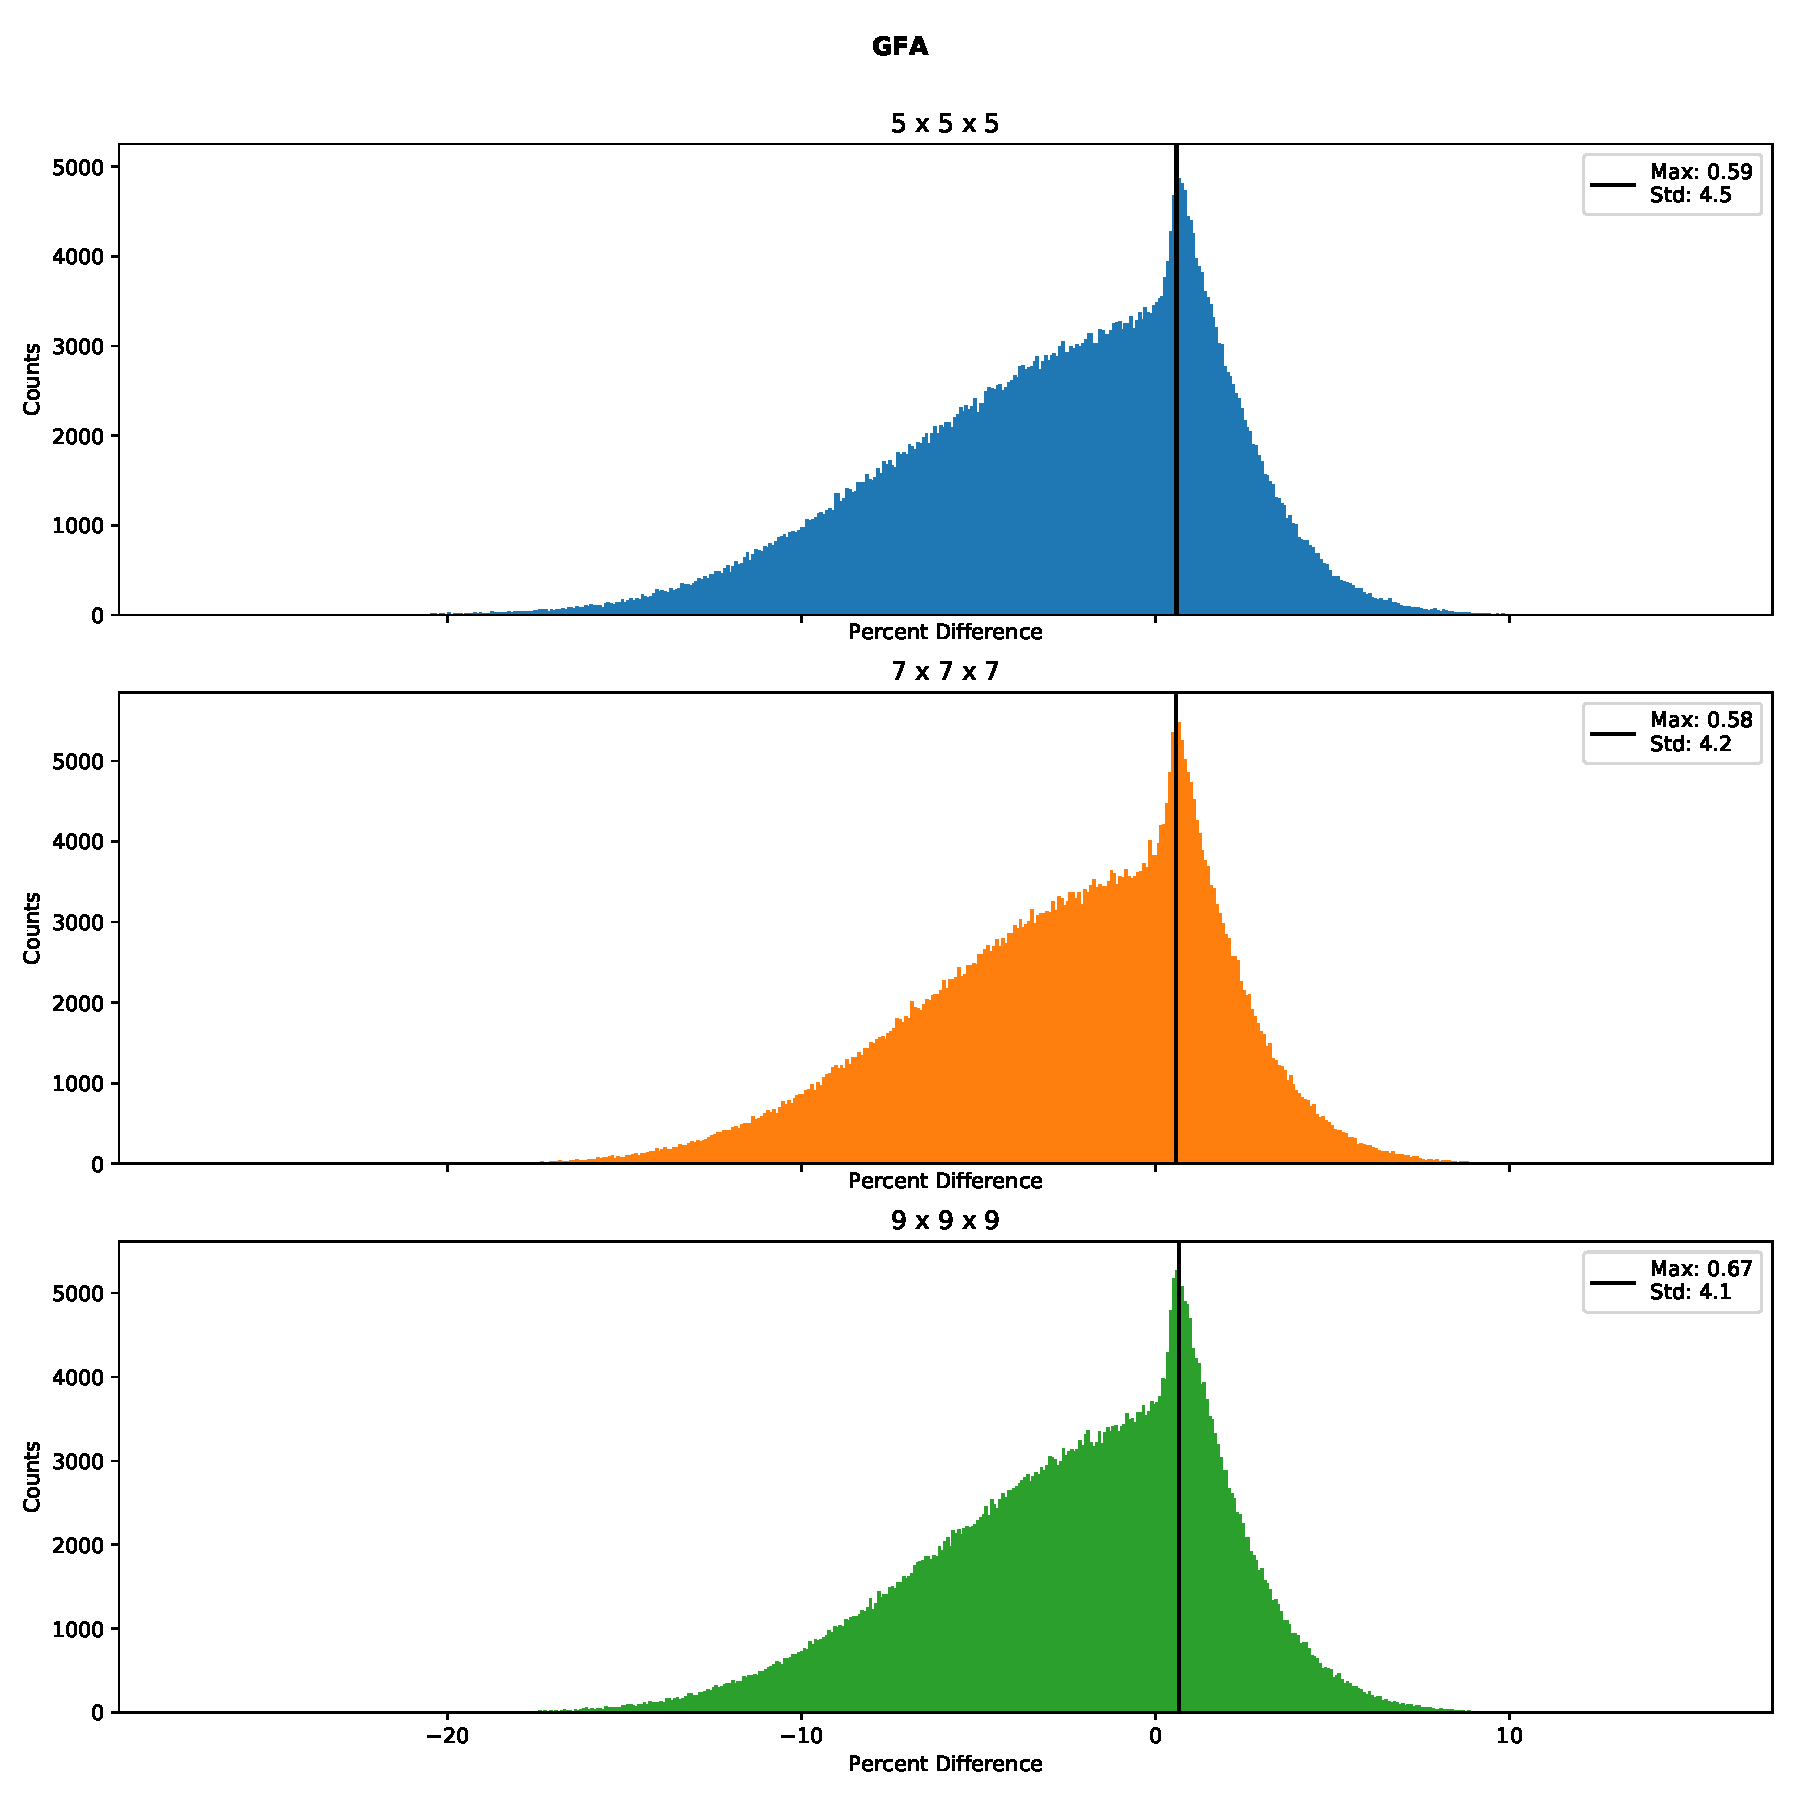
\includegraphics[width=0.6\linewidth]{../figs/gfa}
  \captionsetup{width=0.6\linewidth}
  \caption{Distributions of percent difference in GFA between raw and denoised fODFs.}
  \label{fig:gfa}
\end{figure}

We see that the distributions peak with a difference around 0.6\%, but skew
negative, indicating that the denoised fODFs tend to have a smaller GFA than the
raw fODFs. This agrees with the results from the response function comparison:
the denoised fODFs and response function are more isotropic and have less power
at high angular frequency bands than the raw fODFs. This makes intuitive sense:
high frequency noise in the raw data carries over into high angular frequency
noise in the reconstructed fODF.

%%%%%%%%%%%%%%%%%%%%%%%%%%%%%%%%%%%%%%%%%%%%%%%%%%%%%%%%%%%%%%%%%%%%%%%%
% Number of peaks
%%%%%%%%%%%%%%%%%%%%%%%%%%%%%%%%%%%%%%%%%%%%%%%%%%%%%%%%%%%%%%%%%%%%%%%%
\subsubsection{Number of peaks}
Peaks in the fODFs are defined as points on the fODF that are greater than at
least one neighbor and greater than or equal to all neighbors (a perfectly
isotropic fODF would thus have zero peaks). In this study, peaks were also
filtered by their relative size (only including peaks with height greater than
0.5 of the greatest peak height) and spacing on the sphere (only including peaks
with an angular separation greater than 25 degrees of larger peaks). Additionally,
a maximum of five peaks was found at each voxel.

Figure~\ref{fig:numpeaks} shows the distribution of difference in number
of peaks between the raw and denoised data. For all sliding window widths,
the distributions are symmetric about zero. 

\begin{figure}[H]
  \centering
  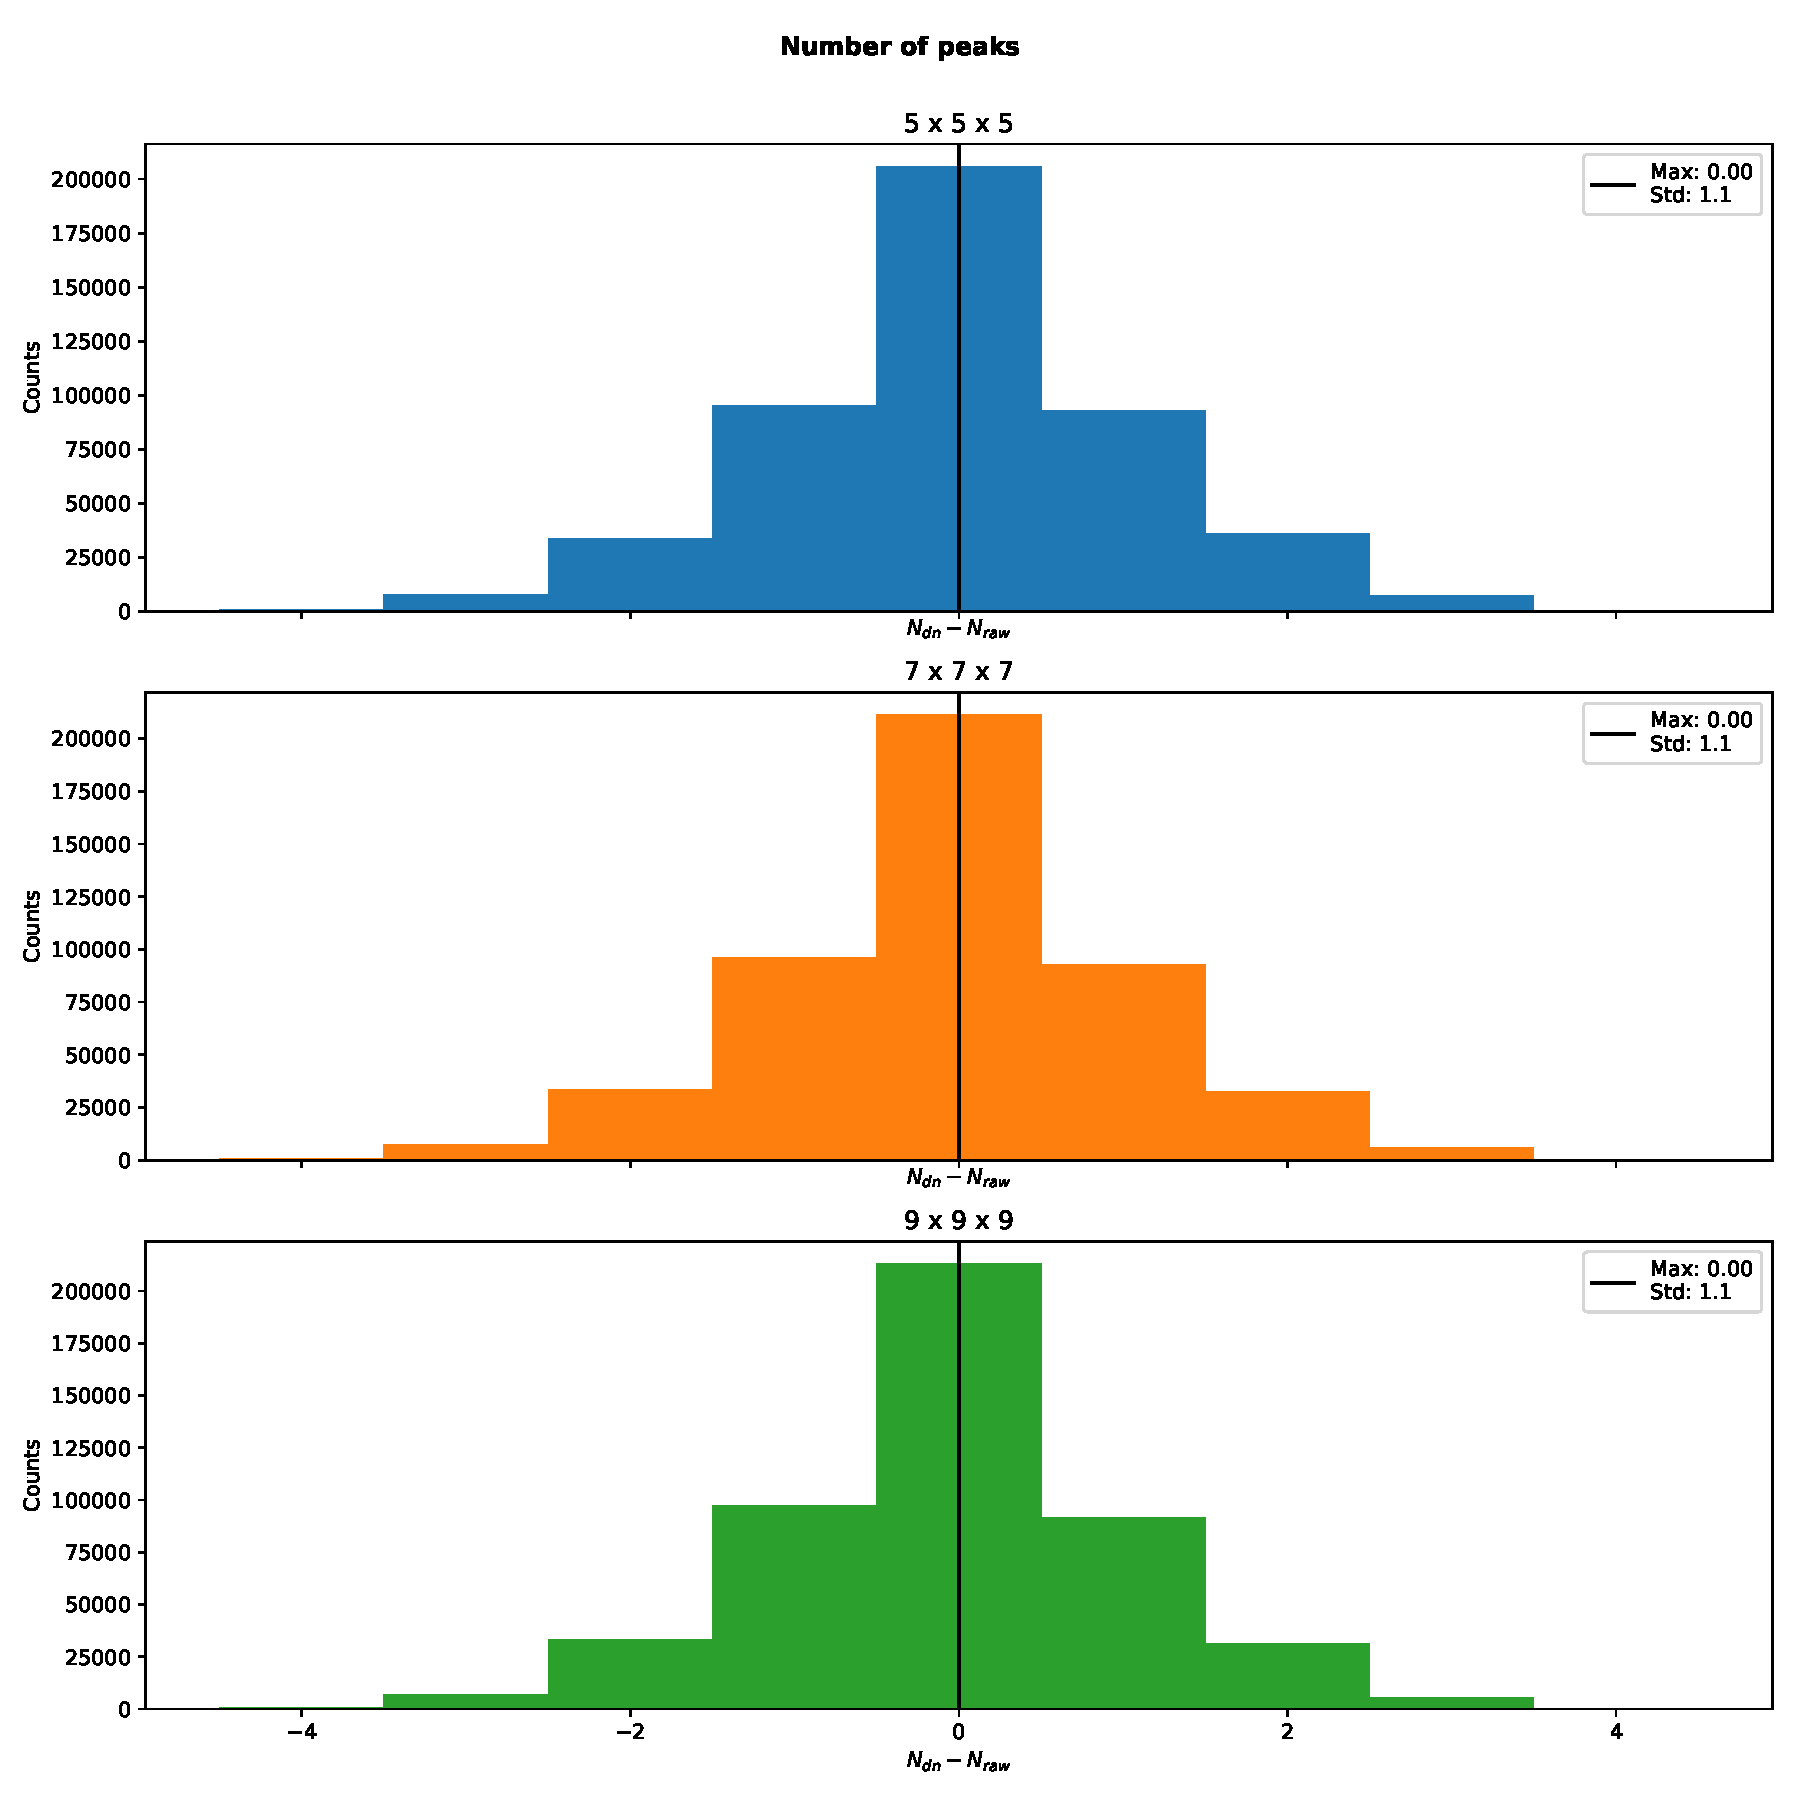
\includegraphics[width=0.6\linewidth]{../figs/numpeaks}
  \captionsetup{width=0.6\linewidth}
  \caption{Distributions of difference in number of peaks between raw and
    denoised fODFs.}
  \label{fig:numpeaks}
\end{figure}

%%%%%%%%%%%%%%%%%%%%%%%%%%%%%%%%%%%%%%%%%%%%%%%%%%%%%%%%%%%%%%%%%%%%%%%%
% Angular separation
%%%%%%%%%%%%%%%%%%%%%%%%%%%%%%%%%%%%%%%%%%%%%%%%%%%%%%%%%%%%%%%%%%%%%%%%
\subsubsection{Angular separation}
Masks were created to only select voxels in which the fODFs for all raw and
denoised volumes had exactly two peaks. Figure~\ref{fig:angdiff} shows the
distribution of angular separations between these peaks in the denoised and raw
volumes. The large gap between the 0$^{\circ}$ bin and the rest of the
distribution is due to the discretization of the sphere. The peak-finding
algorithm used 724 sampling points spaced roughly uniformly across the sphere,
with a mean angular separation distance between neighboring sample points of
7$^{\circ}$ degrees. Accordingly, if the peak-finding algorithm does not place
the peak at the exact same sample point in both fODFs, in most cases it cannot
be placed closer than 7$^{\circ}$.


\begin{figure}[H]
  \centering
  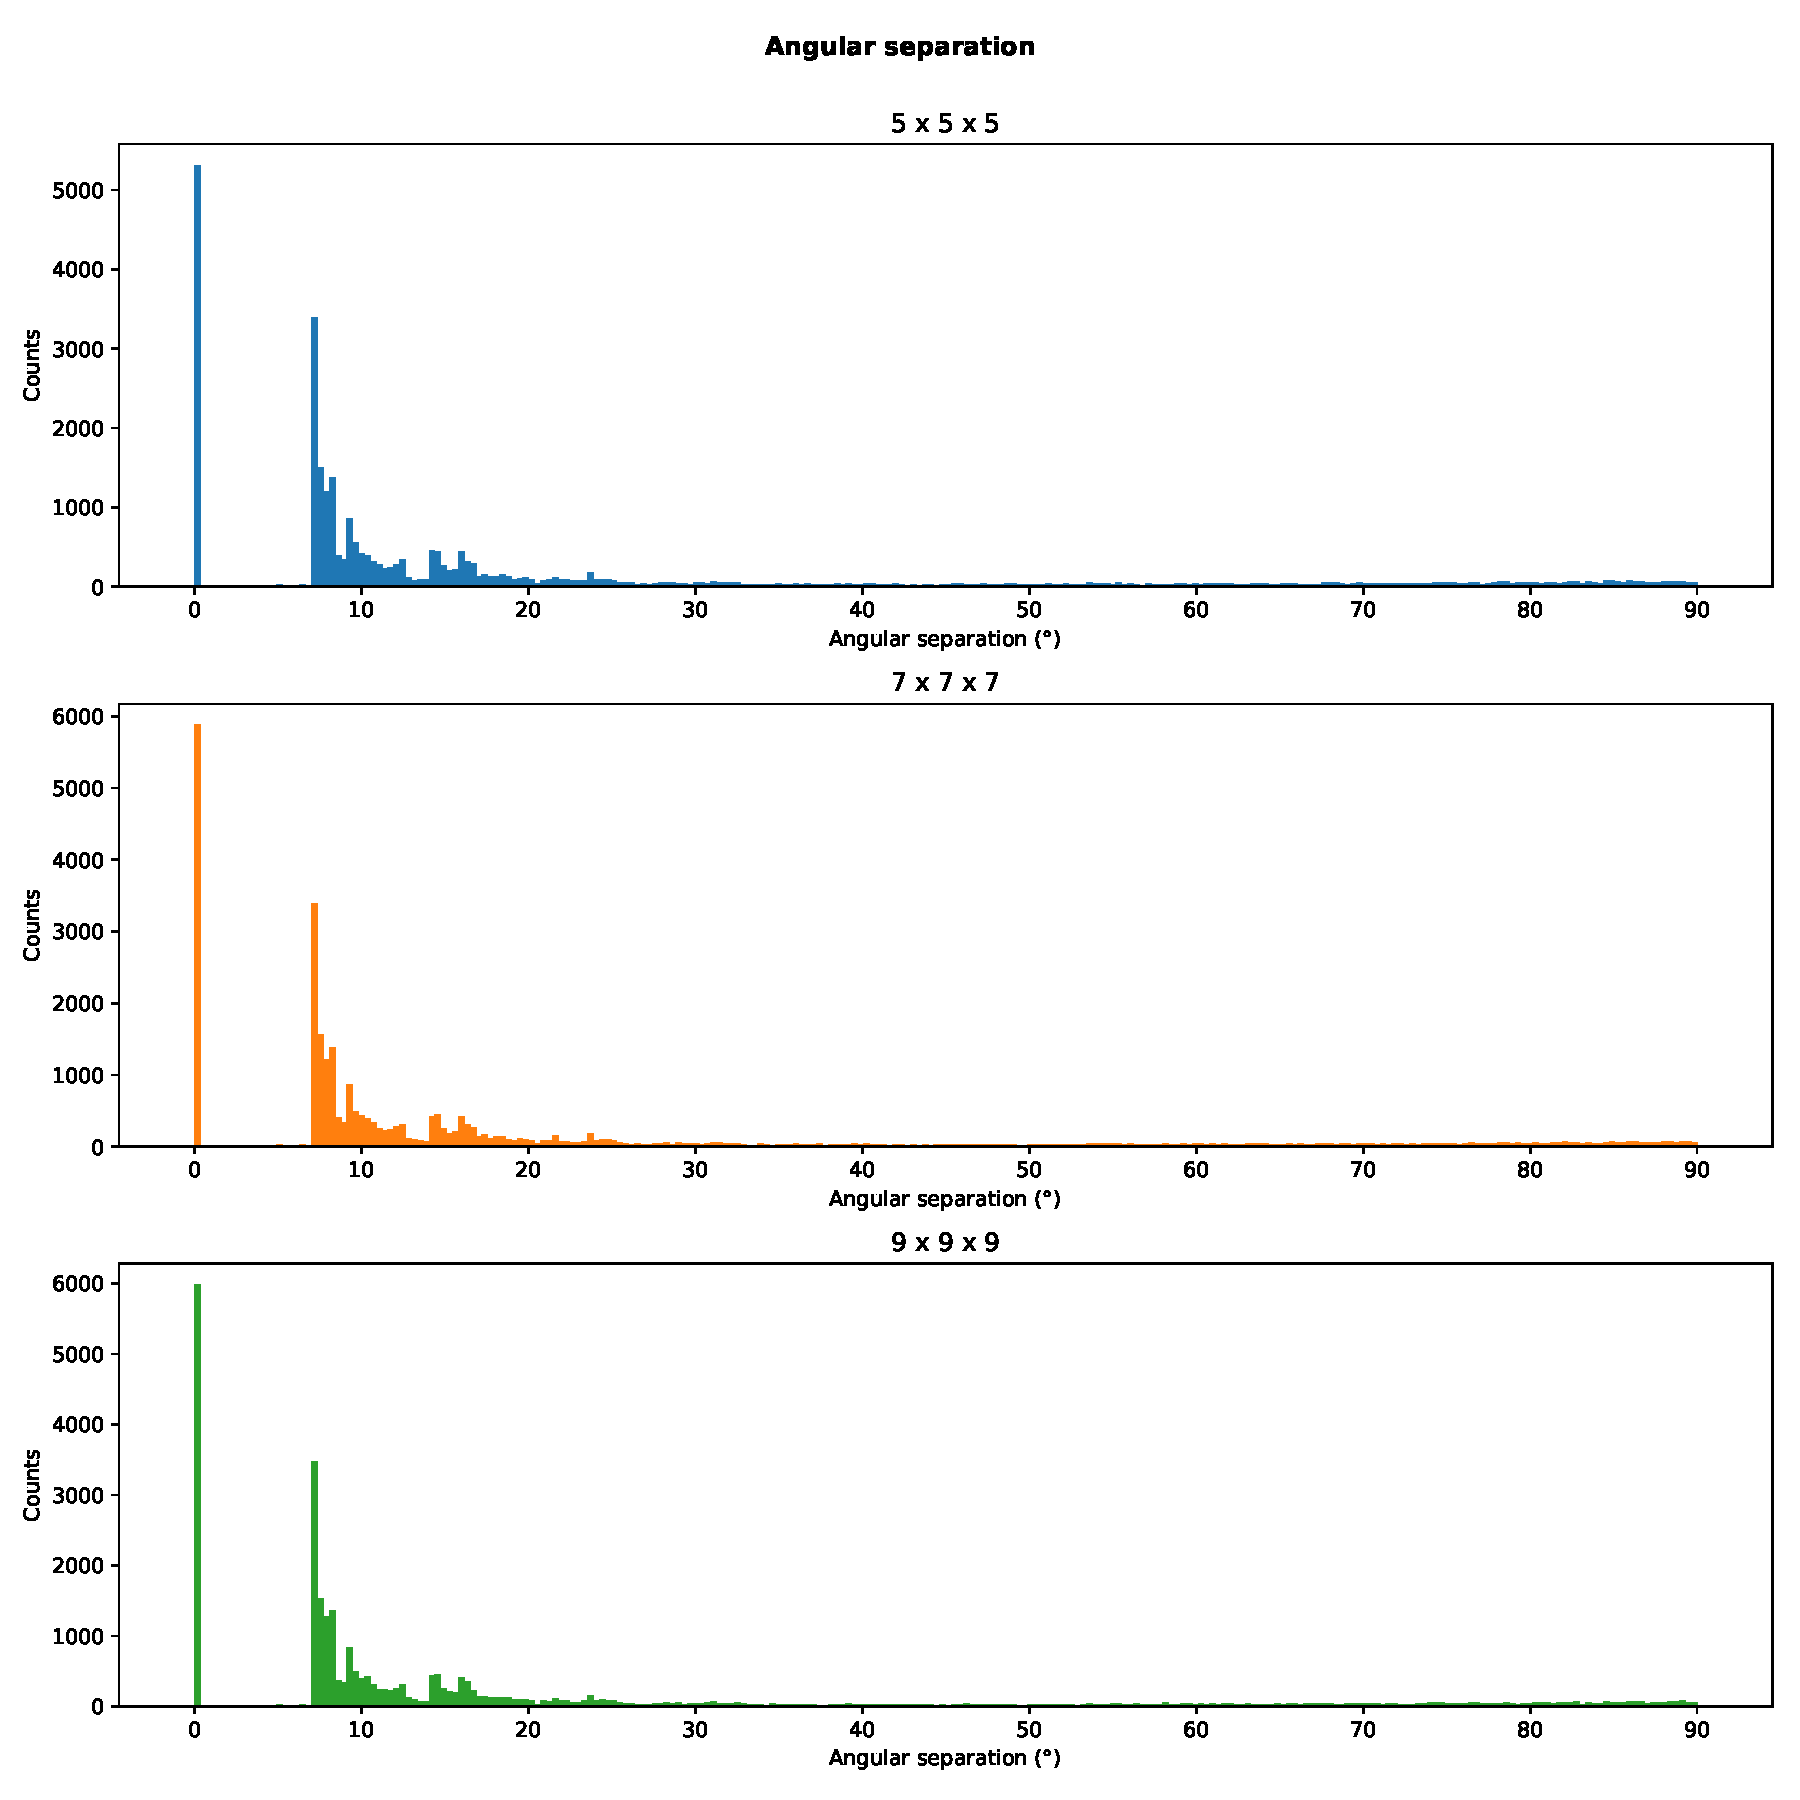
\includegraphics[width=0.6\linewidth]{../figs/angdifference_firsttwo}
  \captionsetup{width=0.6\linewidth}
  \caption{Distributions of angular separation between peaks in the raw and
    denoised fODFs (for fODFs with two peaks).}
  \label{fig:angdiff}
\end{figure}

%%%%%%%%%%%%%%%%%%%%%%%%%%%%%%%%%%%%%%%%%%%%%%%%%%%%%%%%%%%%%%%%%%%%%%%%
% SH Power
%%%%%%%%%%%%%%%%%%%%%%%%%%%%%%%%%%%%%%%%%%%%%%%%%%%%%%%%%%%%%%%%%%%%%%%%
\subsubsection{Angular Frequency Power}

Finally, I looked at the distributions of the percent difference in power in
each spherical harmonic degree, defined as:
\begin{align}
  P_{\ell} = \sum_{m=-\ell}^{\ell} c_{\ell m}^2
\end{align}

Figure~\ref{fig:shpower0} shows these distributions as boxplots at each SH
degree. Generally, the denoised fODFs have more power in the $\ell = 2$ band,
and less or equal power for other bands. Additionally, the variance of the
percent difference in power tends to get larger at higher degree
bands. Figure~\ref{fig:shpower85} shows the same information while only
considering fODFs with GFA $>=$ 0.85. Generally, the percent differences are
closer to zero, with lower variance. 

\begin{figure}[H]
  \centering
  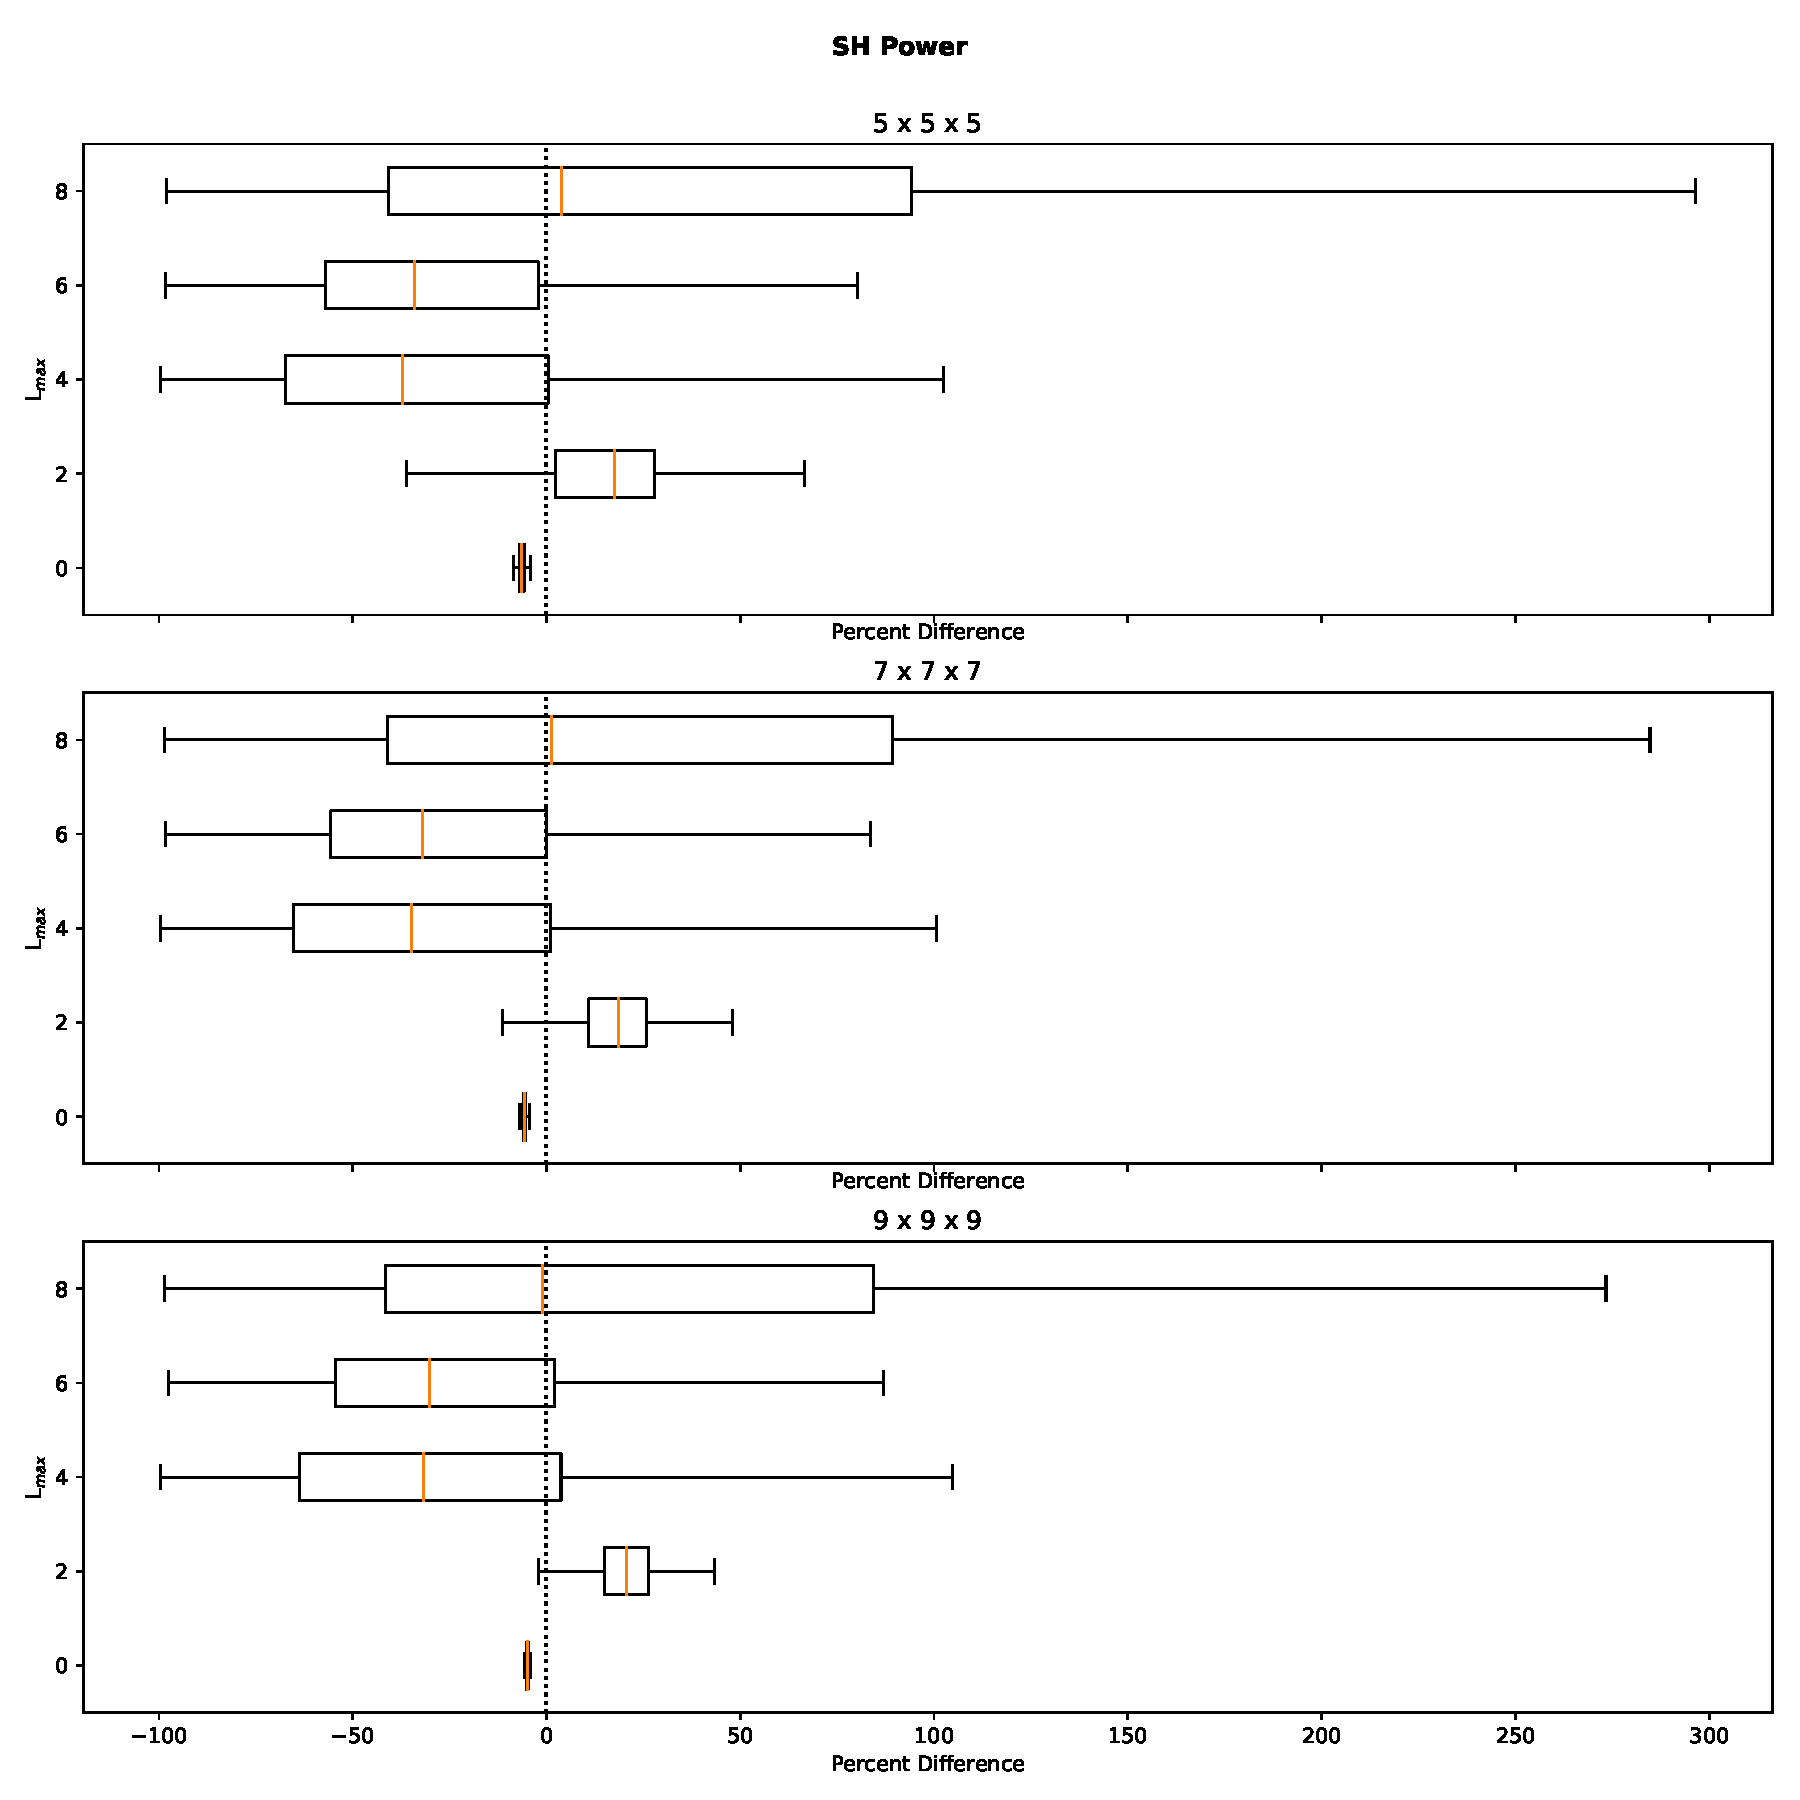
\includegraphics[width=0.5\linewidth]{../figs/shpower_gfa0}
  \captionsetup{width=0.6\linewidth}
  \caption{Distributions of percent differences in power for each SH degree.}
  \label{fig:shpower0}
\end{figure}

\begin{figure}[H]
  \centering
  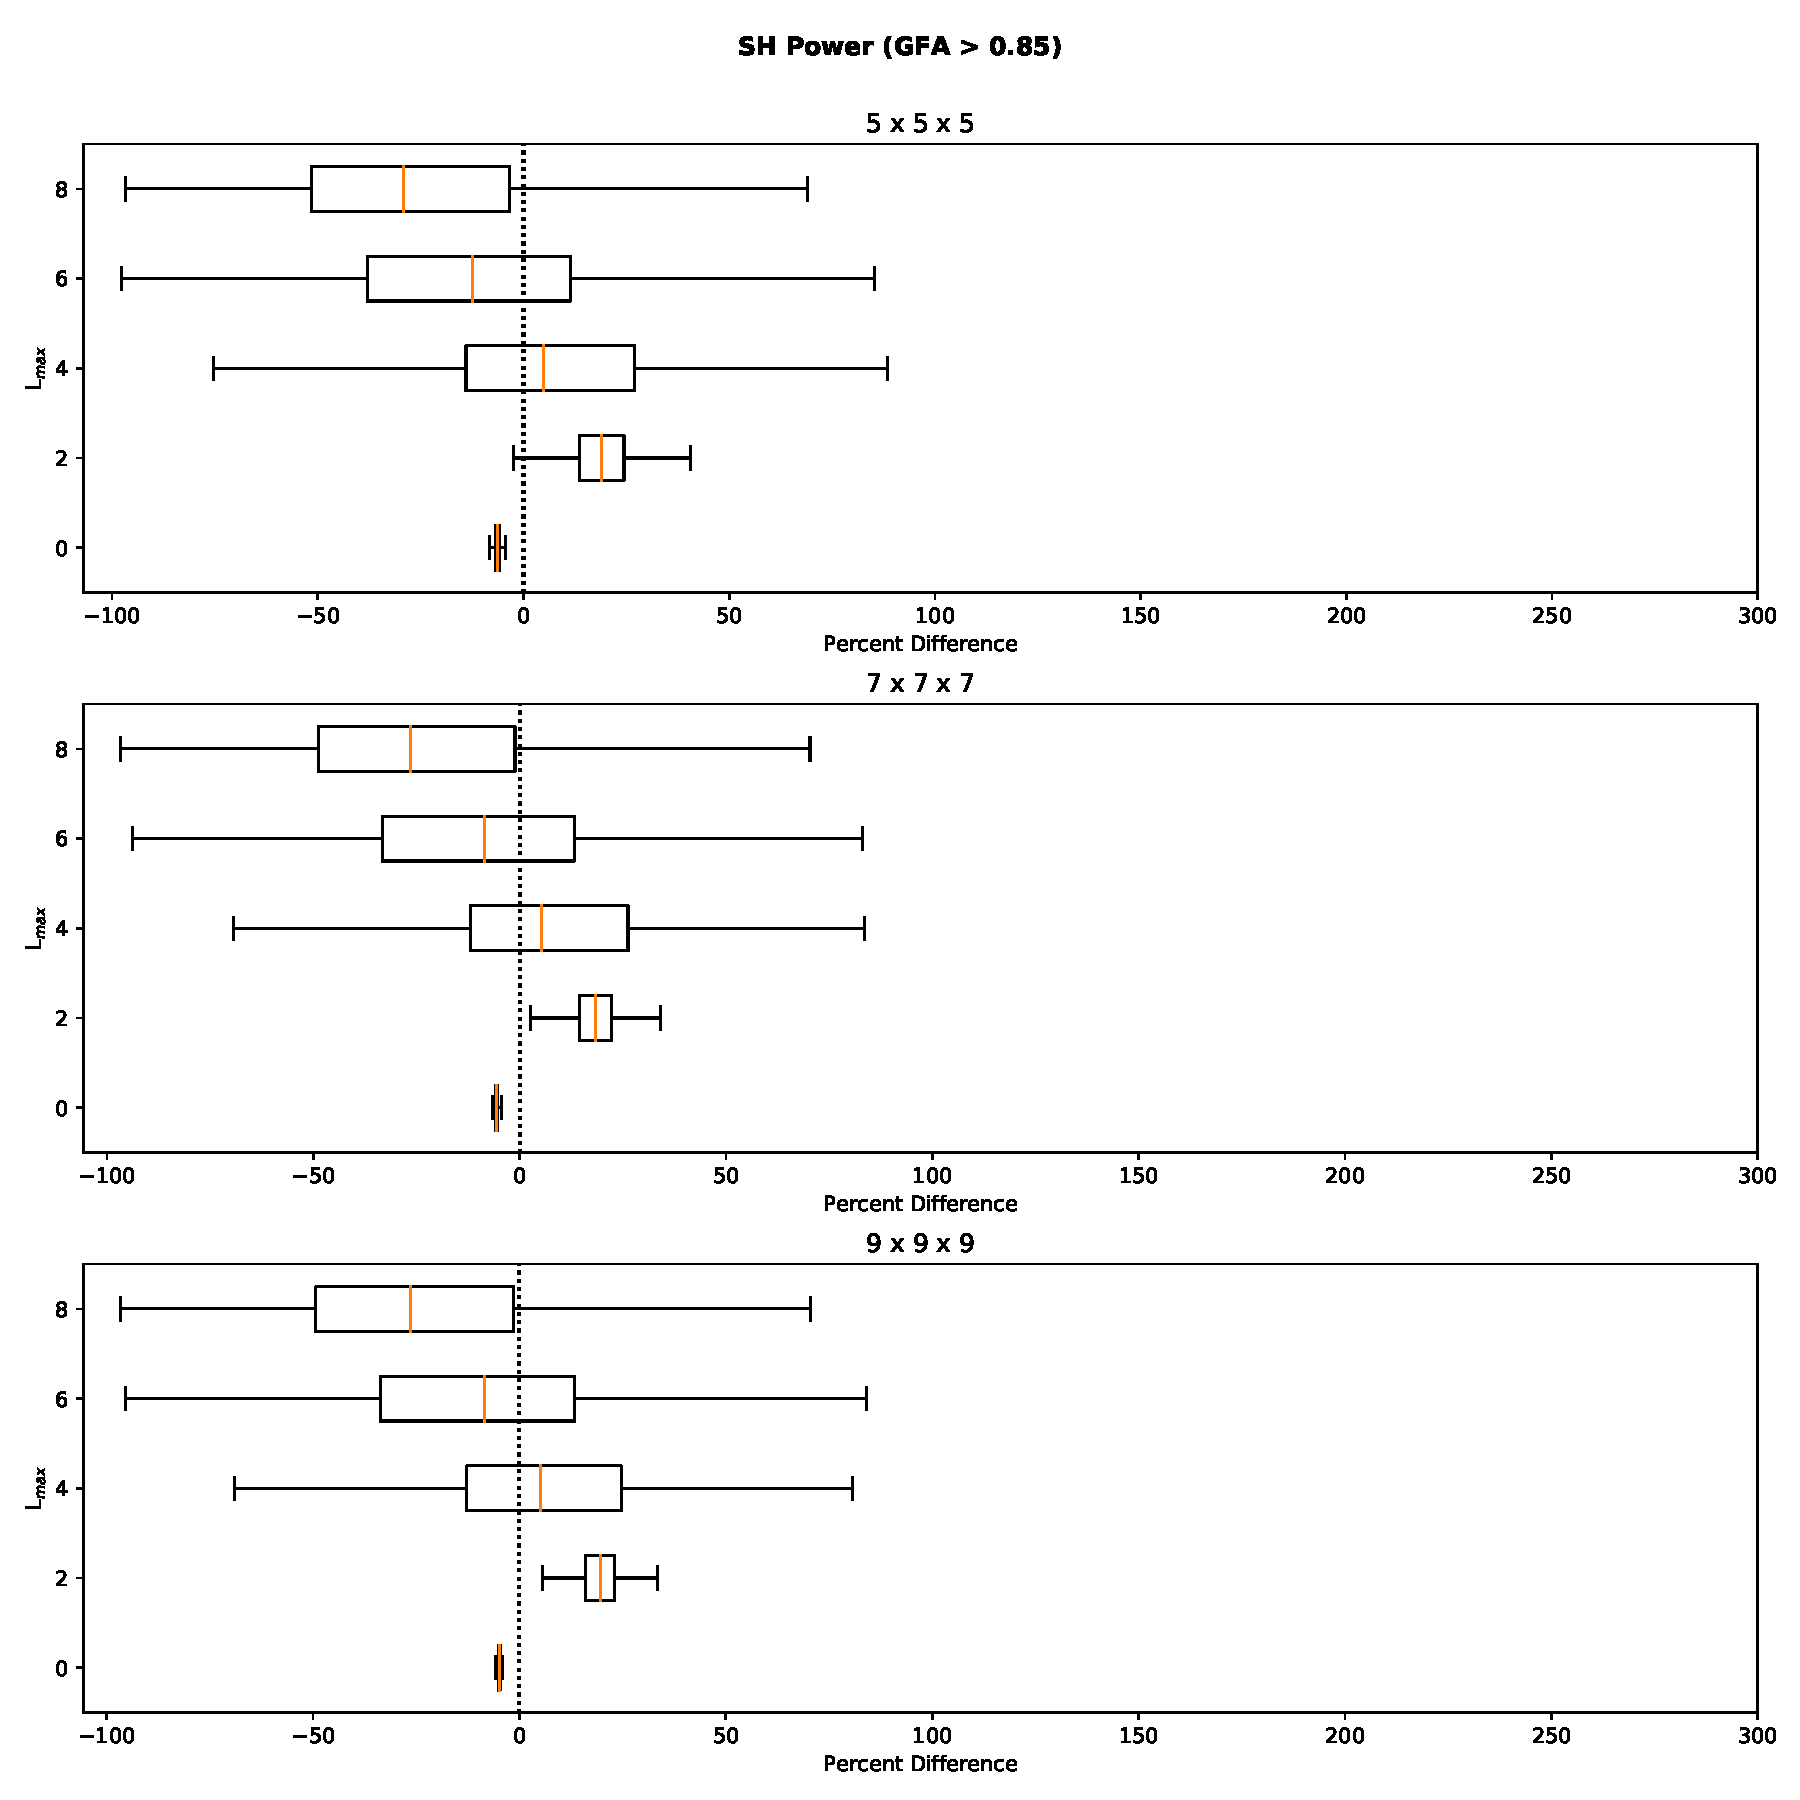
\includegraphics[width=0.5\linewidth]{../figs/shpower_gfa85}
  \captionsetup{width=0.6\linewidth}
  \caption{Distributions of percent differences in power for each SH
    degree. fODFs are restricted to only include those with GFA $>=$ 0.85}
  \label{fig:shpower85}
\end{figure}

\section{Conclusion}
Similarly to the results from the tensor fit, the overall conclusion from these
comparisons is that denoising has some effect on various metrics calculated from
the fODFs, and this effect is not dramatically sensitive to the choice of
sliding window size in the denoising algorithm. Again, without ground truth
fODFs for comparison, we cannot conclude much else about the value of denoising
or the optimal sliding window size.

The next step on this project is to acquire the microCT data and begin working
through any registration challenges, depending on the state of the sample
staining issue. We now have a full CSD reconstruction of the dataset --- if
needed I can look into tractography across the whole brain to identify
potentially important tracts we should avoid if we end up needing to section the
sample prior to x-ray imaging.

\bibliographystyle{ieeetr}
\bibliography{csd_notes}
\end{document}